% ============================================================
% 第4章：系统实现与模块设计
% ============================================================

\section{总体软件流程}

系统以 Python 为核心语言，将 16 个核心模块组织在 \texttt{app/} 目录下，各模块通过 Pydantic IR 数据模型实现松耦合与独立测试。模块组织结构如表 \ref{tab:modules} 所示。

\begin{table}[h]
\centering
\caption{核心模块功能说明}
\label{tab:modules}
\footnotesize
\setlength{\tabcolsep}{6pt} % 调整列间距
\renewcommand{\arraystretch}{1.1} % 调整行高
\begin{tabularx}{\textwidth}{p{4cm}Xp{3.5cm}}
\toprule
\textbf{文件名} & \textbf{功能} & \textbf{在 Pipeline 中的阶段} \\
\midrule
\texttt{schemas.py} & IR 数据模型定义（\texttt{PartIR}、\texttt{RiskIR} 等） & 贯穿全局 \\
\texttt{requirement\_parser.py} & 四级容错需求解析链 & 需求解析 \\
\texttt{ezplm\_client.py} & eZ-PLM API 客户端（HMAC 签名、MPN 电压推断、离线兜底） & 器件检索 \\
\texttt{llm\_client.py} & DeepSeek/OpenAI LLM 调用封装 & 需求解析、混合评分 \\
\texttt{rag.py} & ChromaDB 向量存储与语义检索 & 知识增强 \\
\texttt{scoring.py} & 双模自适应评分引擎、去重与推荐分级 & 混合评分 \\
\texttt{evidence.py} & 八类证据链自动生成 & 证据构建 \\
\texttt{report\_generator.py} & 双层风险评估（13 类规则 + LLM 叙述分离） & 报告生成 \\
\texttt{output\_generator.py} & 风险评估与拓扑分析 Markdown 渲染、\texttt{TopologyIR} JSON & 报告生成 \\
\texttt{output\_bom.py} & BOM 选型清单 Markdown 渲染 & 报告生成 \\
\texttt{agent\_orchestrator.py} & Pipeline 主调度、RAG 触发、参考设计拉取 & 调度层 \\
\texttt{agent\_tools.py} & 4 个 LangChain Tool & Agent 工具层 \\
\texttt{react\_agent.py} & ReAct Agent 创建、会话管理及幻觉检测 & Agent 推理层 \\
\texttt{main.py} & FastAPI 服务入口（5 类端点、CORS 支持） & 服务层 \\
\texttt{log\_util.py} & 调试日志工具 & 辅助模块 \\
\texttt{datasheet\_rag.py} & 数据手册 RAG & 辅助模块 \\
\bottomrule
\end{tabularx}
\end{table}


\section{Pipeline 调度实现}

Pipeline 主入口 \texttt{analyze()} 定义于 \texttt{agent\_orchestrator.py}，将解析、检索、评分、证据构建与报告生成五个阶段串联为端到端执行链路。调度层在检索阶段完成后执行两项增强操作：

\begin{enumerate}
\item 若 LLM 密钥可用，对排名前 10 的 \texttt{ezplm} 来源候选器件调用 \texttt{fetch\_refere\\nce\_designs()}，通过 eZ-PLM 参考设计接口获取每器件最多三条设计案例，构建 \texttt{ref\_designs\_map} 字典供评分引擎使用。
\item 调用 \texttt{\_query\_rag\_knowledge()} 自动触发 RAG 检索，根据用户需求及解析约束构建查询文本，获取 Top-5 条目并以 \texttt{EvidenceIR} 形式注入证据链。
\end{enumerate}

本地处理环节耗时控制在 20 毫秒以内，主要开销集中于 eZ-PLM API 网络请求和 LLM 远程调用，保证了高效的数据流与实时性。

\section{需求解析模块}

\texttt{requirement\_parser.py} 的唯一公开接口为 \texttt{parse\_requirement(text: str) -> RequirementConstraints}。除了第三章 3.1 节中算法原理的介绍，本节从软件实现角度补充两个关键细节：

\begin{itemize}
\item \textbf{LLM 结果归一化}：\texttt{\_norm\_cat()} 和 \texttt{\_norm\_topo()} 将 LLM 输出的多样化表述统一为标准值（如 \texttt{"DC-DC"、"降压"、"电源管理"} 归一化为 \texttt{dc\_dc\_con\\verter}），避免后续匹配失效。
\item \textbf{规则覆盖策略}：规则引擎仅在已验证的缺陷场景下定向修正——关键词匹配仅在出现 \texttt{"降压"、"buck"、"升压"、"boost"、"ldo"} 时触发，电压比较仅在 DC-DC 且电压均提取时生效，mA 匹配与否定句式处理仅在特定正则匹配时执行。该策略保留 LLM 对自然语言的理解优势，同时保证关键参数的工程可靠性。
\end{itemize}

\section{器件检索模块}

\texttt{ezplm\_client.py} 实现“API 优先、离线兜底”双路径策略，核心接口 \texttt{search\_\\parts()}。模块遍历 \texttt{\_API\_KEYWORDS} 映射表将类别/拓扑映射至制造商前缀（如 Buck 对应 TPS54、LM2596 等），每前缀发 HMAC-SHA256 签名 GET 请求（最多 50 条，总召回 200 条），返回 JSON 经 \texttt{\_map\_api\_part\_to\_partir()} 转为 \texttt{PartIR}，再通过五维过滤（类别、电压覆盖、$\pm 5\%$ 输出电压容差、电流下限、温度/等级匹配）生成候选列表。

\section{混合评分与 LLM 调用模块}

混合评分引擎（\texttt{scoring.py}）核心接口为 \texttt{score\_candidates()}，依次计算参数匹配分和供应链稳定性分后，根据参考设计数据可用性选择纯规则或 LLM 增强模式。双模加权公式与子维度打分函数见第三章第 3.3 节。评分完成后，\texttt{\_extract\_core\_mpn()} 对同系列变体去重合并并按 Top-N 策略截断。

LLM 调用模块（\texttt{llm\_client.py}）通过读取环境变量动态适配 OpenAI 兼容端点，实现 DeepSeek、GPT、Claude 等模型的无缝切换。模块提供 \texttt{parse\_require\\ment\_with\_llm()} 和 \texttt{score\_part\_with\_llm()} 两个专用函数，分别用于需求解析和 LLM 增强评分，提示词模板内嵌函数体并以系统/用户两级提示词设定角色边界与结构化上下文。

\section{证据构建模块}

证据构建模块（\texttt{evidence.py}）公开接口为 \texttt{build\_evidence()}，遍历评分结果为每个候选器件生成八类证据条目：输入电压覆盖、输出电流满足、温度范围覆盖、库存水平、生命周期状态、车规认证、国产化标识和数据手册可用性。其中，库存为零、停产状态、车规不匹配和无数据手册四类异常触发 \texttt{need\_human\_review} 标记并降低置信度。

\section{报告生成模块}

报告生成模块由 \texttt{output\_bom.py} 与 \texttt{output\_generator.py} 协同实现。\texttt{genera\\te\_bom()} 生成符合 IPC 命名习惯的 BOM 选型清单，包含推荐器件表、备选器件表、关键参数对比矩阵和评分方法说明；

\texttt{output\_generator.py} 的 \texttt{generate\_risk\_report()} 将 \texttt{RiskItem} 列表展开为符合 ISO 31000 框架的 Markdown 文档，包含执行摘要、$5\times 5$ 风险矩阵、供应链/工程风险详述、人工复核清单和结论建议，每条风险均附带数据来源声明以区分规则事实与 LLM 叙述。

\section{ReAct Agent 交互模块}

Agent 交互模块由 \texttt{agent\_tools.py} 和 \texttt{react\_agent.py} 协同实现。\texttt{agent\_to\\ols.py} 基于 LangChain \texttt{@tool} 装饰器定义四个专用工具：\texttt{search\_components}（封装 Pipeline 选型分析）、\texttt{query\_design\_knowledge}（RAG 知识库检索）、\texttt{find\_alternative\_parts}（替代器件查找）和 \texttt{generate\_full\_report}（触发报告生成），每个工具均含自然语言描述和参数 Schema。

\texttt{react\_agent.py} 的 \texttt{create\_component\_agent()} 将上述工具注册到 ReAct Agent 实例，通过系统提示词约束工具调用边界（搜索至多一次、知识检索至多一次、总调用不超过五次），并禁止编造不存在的器件型号以降低幻觉风险。\texttt{run\_agent()} 通过全局会话字典维护多轮对话上下文，递归深度限制为 \texttt{recursion\_limit=8} 以保证响应时延可控。

此外，\texttt{\_validate\_part\_numbers\_in\_response()} 在 Agent 回复前对型号进行数据库交叉校验，若某型号不符合制造商前缀白名单且不在离线数据库中，则在回复末尾追加风险提示以缓解型号幻觉。

\section{Web 服务与前端展示}

Web 服务层（\texttt{main.py}）基于 FastAPI 框架向外暴露第~\ref{sec:architectrue}节所述五个核心端点，通过 \texttt{RequestValidationError} 异常处理器统一处理格式校验与 UTF-8 中文编码兼容问题。

前端展示层（\texttt{frontend/streamlit\_app.py}）基于 Streamlit 框架构建选型交互界面。用户提交自然语言需求后，前端以工具调用步骤卡片实时展示 Pipeline 各阶段进度，评分结果以推荐/备选/不推荐三级可折叠面板呈现（含综合得分进度条、五维子评分项、关键参数速览和评分原因标签），证据链与参数对比整合为一个增强面板，支持按器件型号筛选证据条目并以表格横向对比全部候选器件的关键电气参数。
\begin{figure}[h]
\centering
\includegraphics[width=0.75\textwidth]{figures/前端展示.png}
\caption{前端UI界面}
\label{fig:parse_accuracy}
\end{figure}
\begin{figure}[h]
\centering
\includegraphics[width=0.75\textwidth]{figures/点击Run Analyze.png}
\caption{点击Run Analyze 执行结果}
\label{fig:parse_accuracy}
\end{figure}
\begin{figure}[h]
\centering
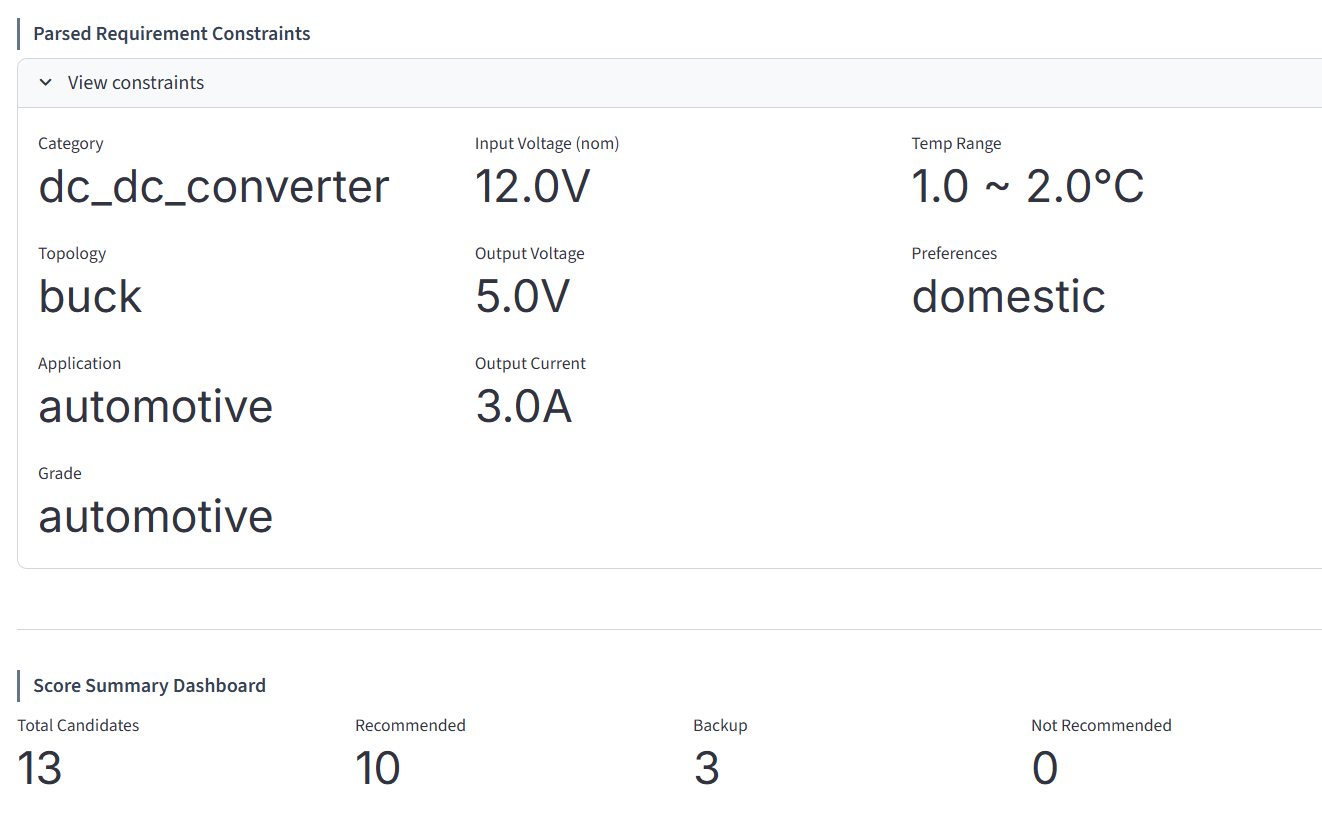
\includegraphics[width=0.75\textwidth]{figures/约束.png}
\caption{约束}
\label{fig:parse_accuracy}
\end{figure}
\begin{figure}[h]
\centering
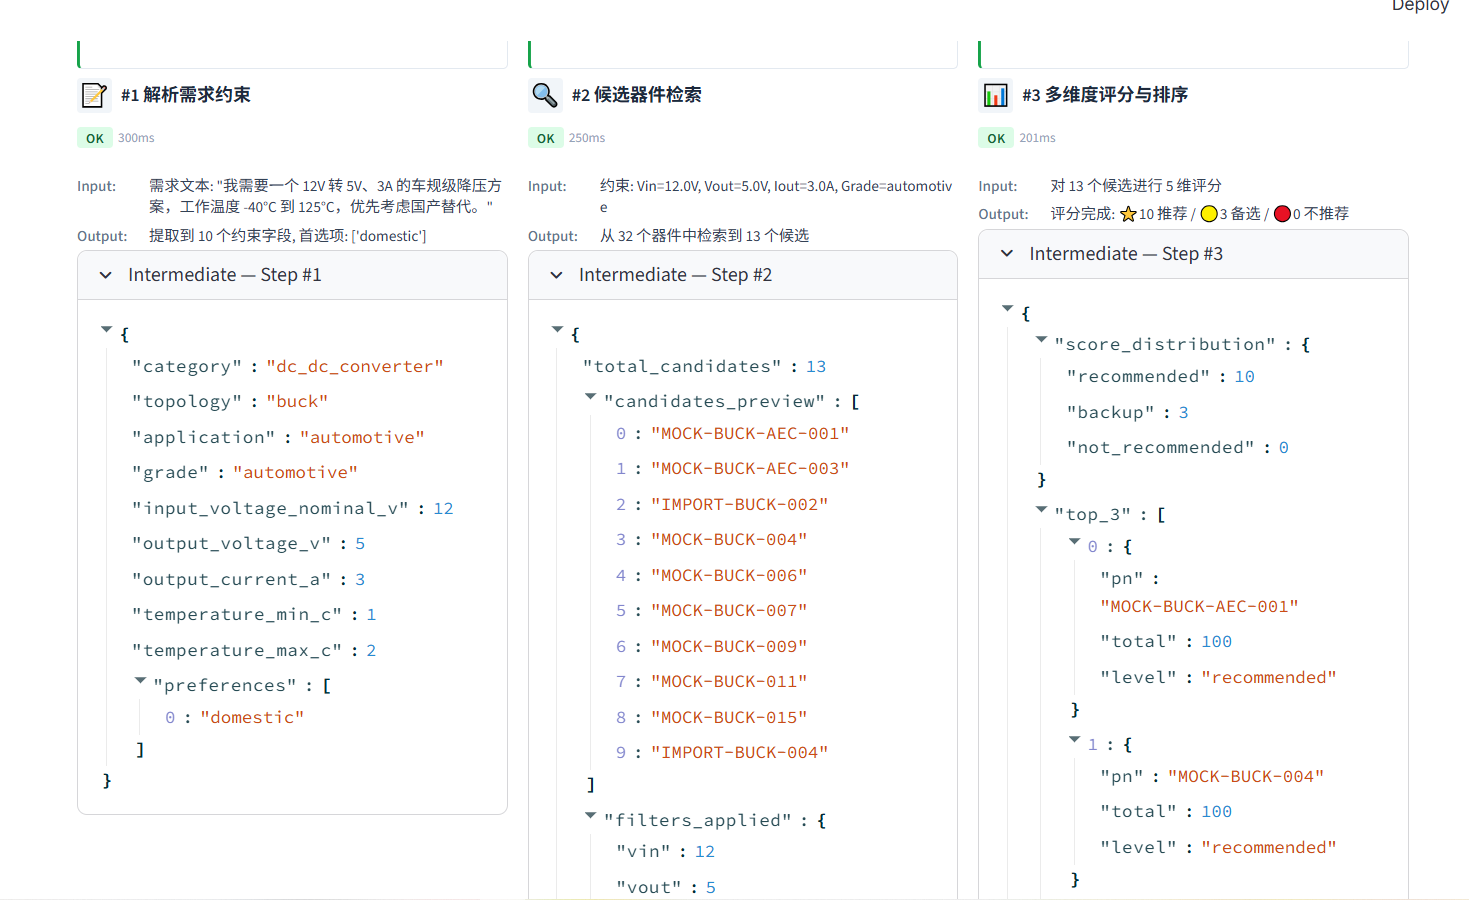
\includegraphics[width=0.75\textwidth]{figures/折叠卡片.png}
\caption{折叠卡片}
\label{fig:parse_accuracy}
\end{figure}
\begin{figure}[h]
\centering
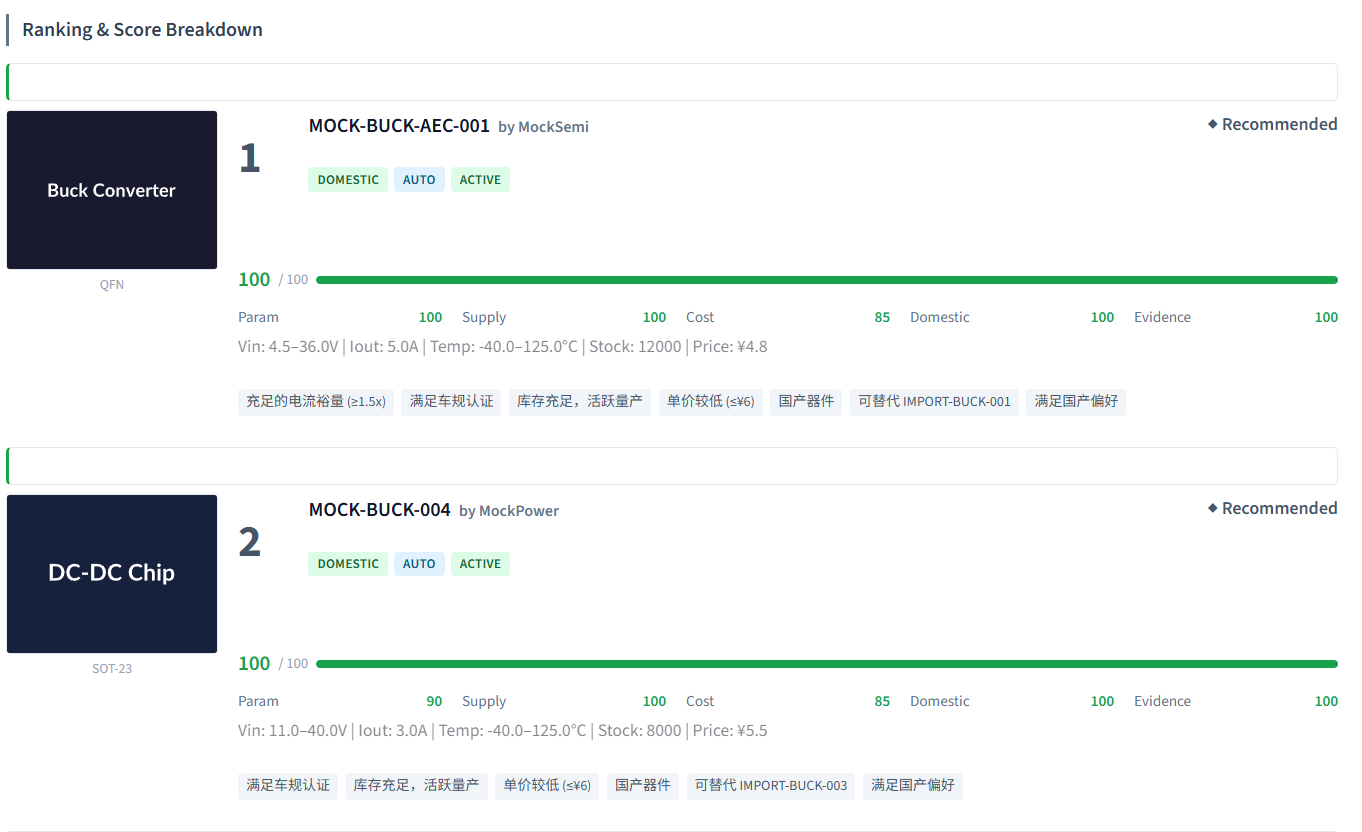
\includegraphics[width=0.75\textwidth]{figures/推荐.png}
\caption{推荐结果}
\label{fig:parse_accuracy}
\end{figure}
\begin{figure}[h]
\centering
\includegraphics[width=0.75\textwidth]{figures/选择报告.png}
\caption{选择报告}
\label{fig:parse_accuracy}
\end{figure}
\begin{figure}[h]
\centering
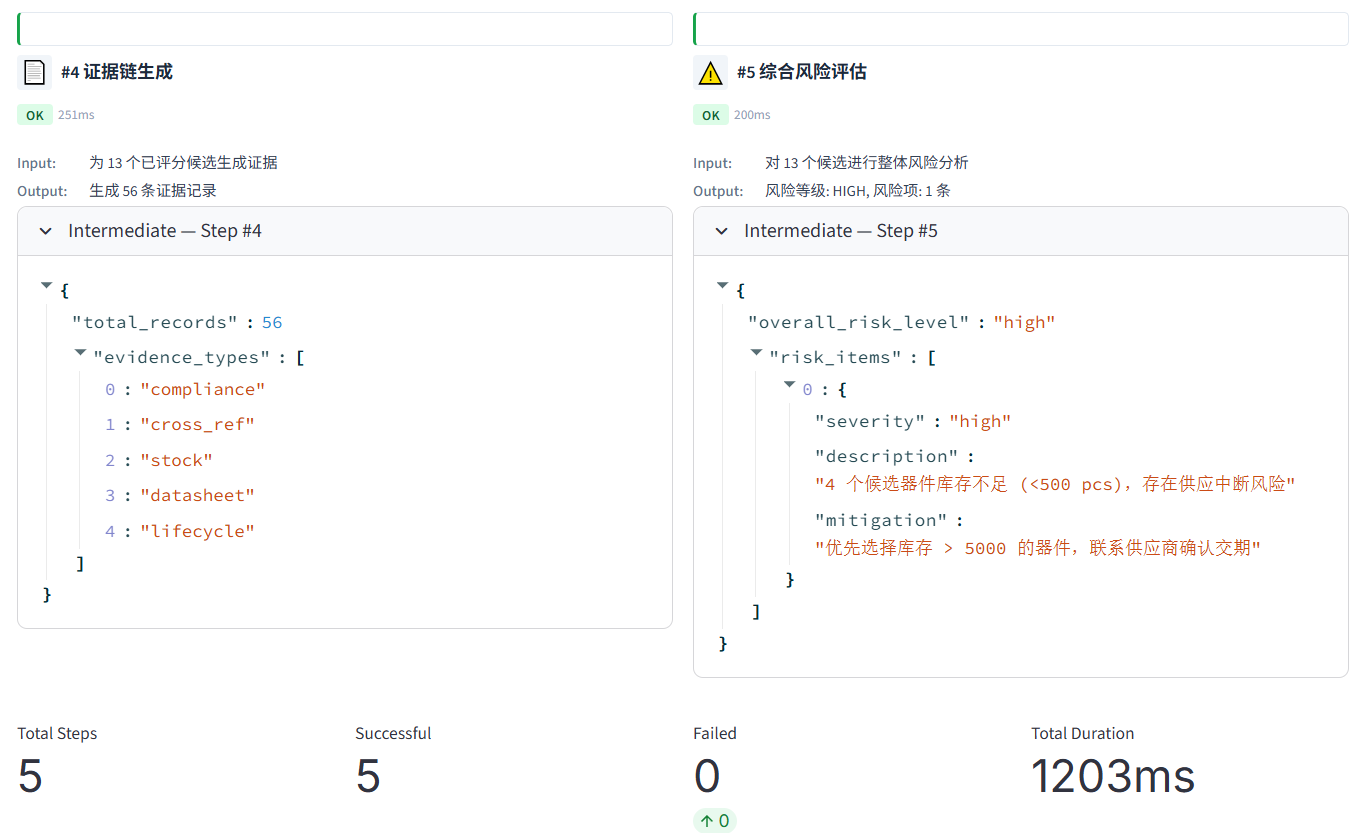
\includegraphics[width=0.75\textwidth]{figures/证据链与综合评估.png}
\caption{证据链与综合风险评估}
\label{fig:parse_accuracy}
\end{figure}
\begin{figure}[h]
\centering
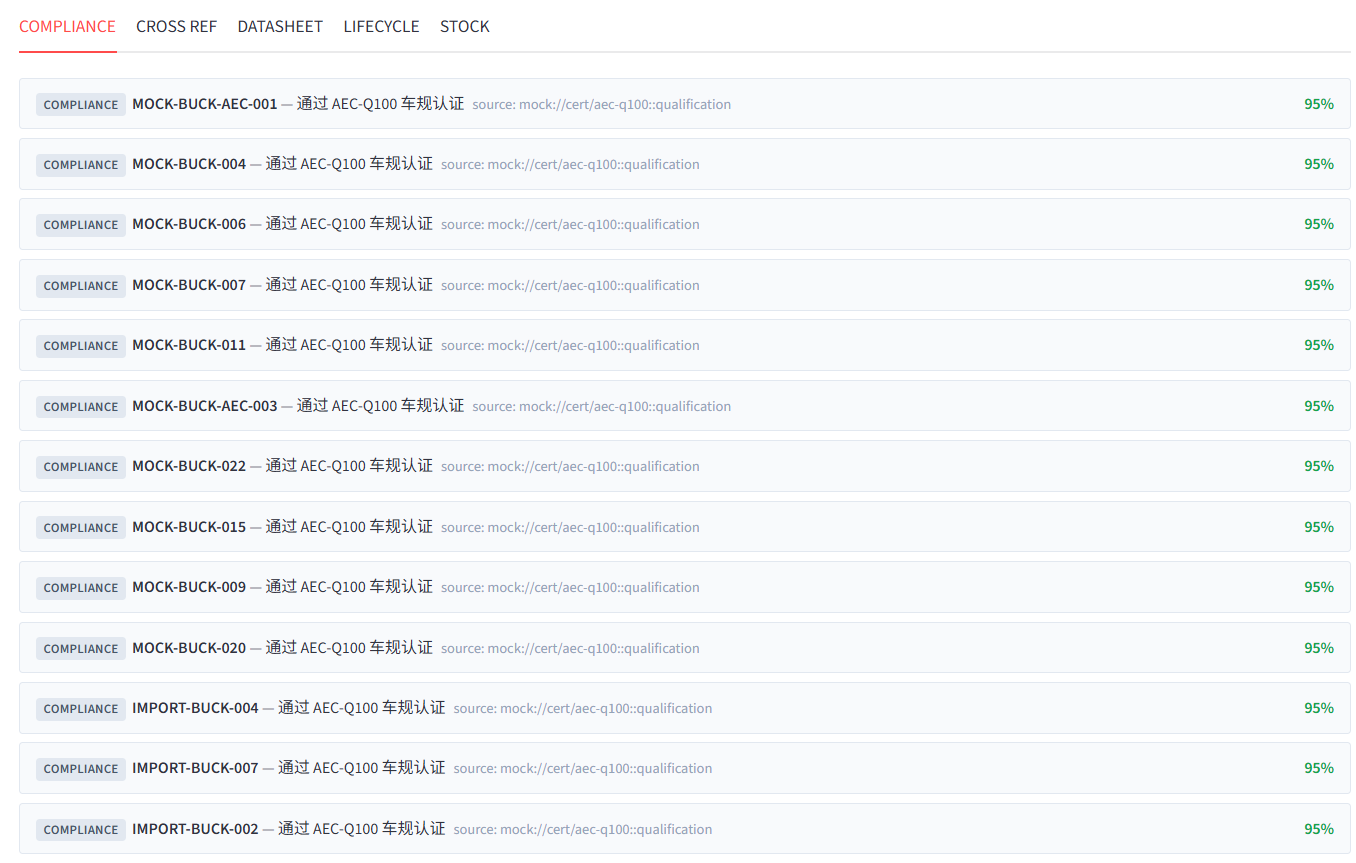
\includegraphics[width=0.75\textwidth]{figures/compliance.png}
\caption{合规}
\label{fig:parse_accuracy}
\end{figure}
\begin{figure}[h]
\centering
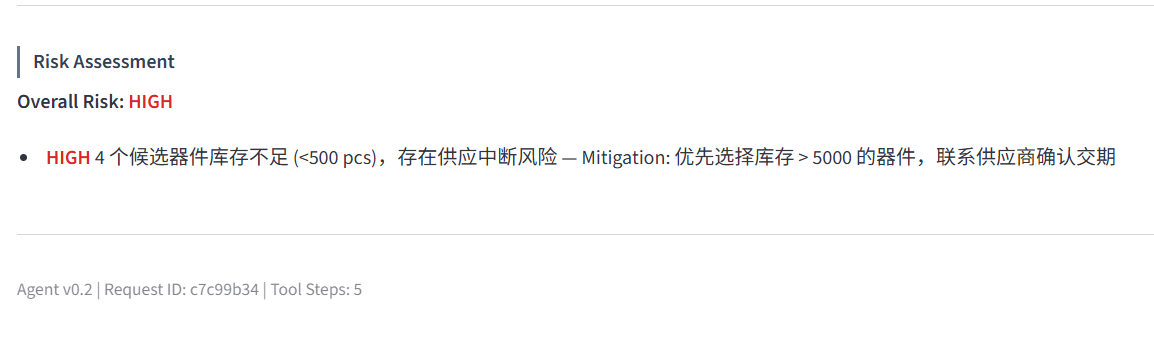
\includegraphics[width=0.75\textwidth]{figures/风险评估.png}
\caption{风险评估}
\label{fig:parse_accuracy}
\end{figure}